\documentclass[12pt,journal,compsoc,onecolumn]{IEEEtran}
\newcommand\MYhyperrefoptions{bookmarks=true,bookmarksnumbered=true,
pdfpagemode={UseOutlines},plainpages=false,pdfpagelabels=true,
colorlinks=true,linkcolor={black},citecolor={black},pagecolor={black},
urlcolor={black},
pdftitle={Bare Demo of IEEEtran.cls for Computer Society Journals},%<!CHANGE!
pdfsubject={Typesetting},%<!CHANGE!
pdfauthor={Michael D. Shell},%<!CHANGE!
pdfkeywords={Computer Society, IEEEtran, journal, LaTeX, paper,
             template}}%<^!CHANGE!
\hyphenation{op-tical net-works semi-conduc-tor}
\usepackage{pdfpages}
\usepackage{float}
\usepackage[center]{caption}

\pagestyle{headings}
\begin{document}
\title{Thesis Outilne}
\author{Cecil Li}

% The paper headers
\markboth{Revision 4\hspace{6cm}Thesis outline}{}
% make the title area
\maketitle
% Revision control
\begin{center}
    \begin{tabular}{ | l | l | l | p{8cm} |}
    \hline
    Revision & Time & Made by & Comments \\ \hline
    1 & 30 Jan 2014 & Cecil Li & Drafted revision 1 from meeting notes.\\ \hline
    2 & 4 Feb 2014 & Cecil Li & Added drawing \ref{fig:Drawing1.jpg} Preprocessing and Analysis Design\\ \hline
    3 & 18 Feb 2014 & Cecil Li & Modified drawing \ref{fig:Drawing1.jpg} to adjust the change in experiment design.\newline    Added Table \ref{table:duedates} for keeping track of work.\\ \hline
    4 & 25 Feb 2014 & Cecil Li & Added Section \ref{Subsection:analysisstage} Analysis \\ \hline
    \end{tabular}
\end{center}
\newpage
\section{Introduction}
\begin{itemize}
\item
State the problem of water availability in agriculture, from literature review. Paraphrase and elaborate.
\item
Introduce the structure of this thesis, explain what are the individual sections.
\end{itemize}

\section{Study of Water Balance Model}
\begin{itemize}
\item
Other people's work on Water balance model
\item
Explain the water balance model and where is it used
\item
Limitations of this model
\item
Briefly introduce the datasets being used, due to the need to spatial data
\end{itemize}

\section{Data Integration}
\begin{itemize}
\item
Explain the datasets: SILO, AWAP, MODIS, DED, LandSAT, etc.
	\begin{itemize}
	\item
	What are them?
	\item
	How to access?
	\item
	Preprocessing data(reprojection, normalization etc.)
	\end{itemize}
\item
Integrate multiple datasets: the i-EKbase system
\item
2 data representation
	\begin{itemize}
	\item
	Point-based
	\item
	Spatial data representation
	\item
	Talk about the temporal resolution and the spatial resolution
	\end{itemize}
\end{itemize}

\section{Mobile App decision support system}
\begin{itemize}
\item
Point-based analysis, its purpose and application
\item
Diagrams, the flow, components
\item
Machine learning approach
\item
Visualisation
\end{itemize}

\section{Area-wise analysis}
\begin{itemize}
\item
Introducing DED and how it improves the spatial resolution
\item
Methods of integrating multiple datasets with DED, interpolation or/and ML technique to improve resolution
\item
Analytics with various ML algorithm, experiments and results
	\begin{figure}[H]
	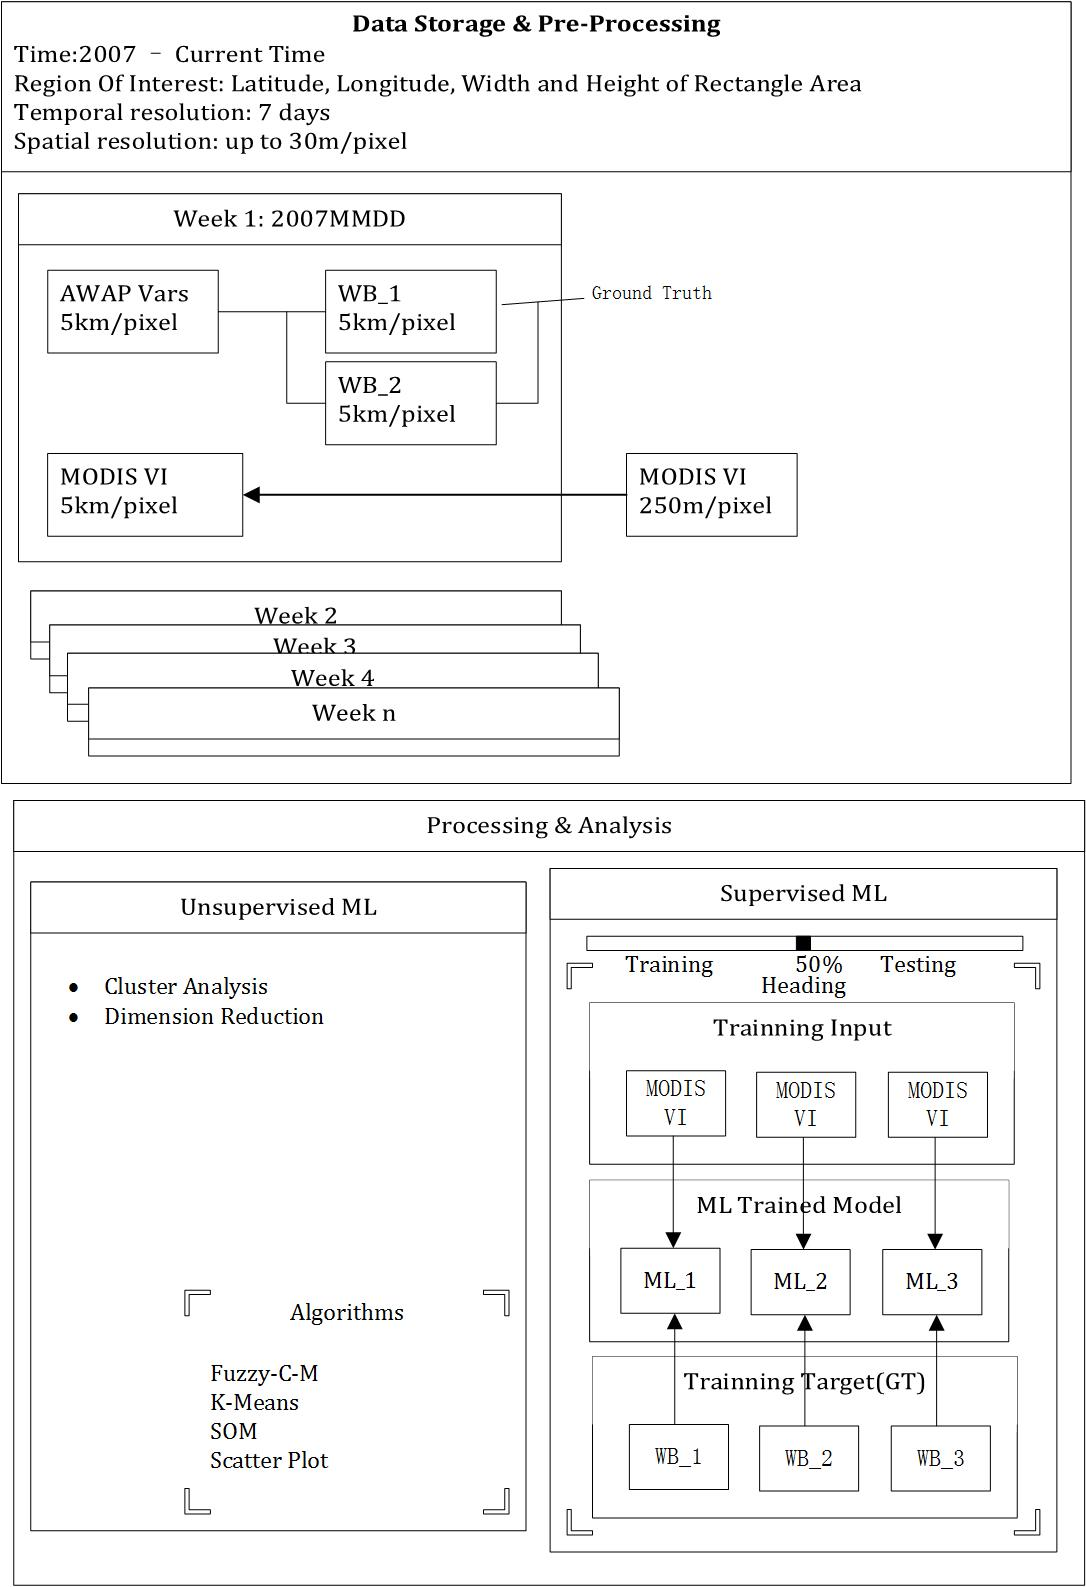
\includegraphics[width=15cm]{Drawing1.jpg}
	\caption{Preprocessing and Analysis Design}\label{fig:Drawing1.jpg}
	\end{figure}
\item
Visualisation of data
\item
Practical application with the customer: Houston farm case study
\end{itemize}
\subsection{Analysis}\label{Subsection:analysisstage}
\subsubsection{Cross Validation of MODIS VI with Landsat Bands}
\begin{enumerate}
\item
Filtering Landsat data by thresholding its cloud-cover level.
\item
Use formula to calculate VI with different band values from Landsat. (Do literature)
\item
Extract Landsat data(30m resolution) for the available MODIS data points(250m resolution), then normalize.
\item
Use established method to find correlation of MODIS VI and Landsat calculated VI(GT)
\item
Analyse the results and draw conclusions. Find out whether MODIS VI is a accurate derived product for vegetation index, if not why.
\end{enumerate}

\subsubsection{High resolution Spatial estimation of water balance}
\begin{enumerate}
\item
Use formula to calculate Water Balance with multiple variables from AWAP. (Do literature)
\item
Extract MODIS data(250m resolution) for the available AWAP data points(5km Resolution)
\item
Supervised Machine Learning Approach:
\begin{itemize}
\item
Training Input: MODIS VI, Digital Elevation Data
\item
Training Target: AWAP calculated Water Balance Value
\item
Testing Input: MODIS VI, DED
\item
Testing Target: AWAP calculated Water Balance Value (Historic Data)
\end{itemize}
Unsupervised Machine Learning Approach:
\begin{itemize}
\item
Training Input: AWAP calculated Water Balance
\end{itemize}
\item
Analyse the results, the precision of the model's estimation
\item
If acceptable, deploy the algorithm to data points where MODIS VI and DED are available whereas AWAP is not, at a resolution of 250m/pixel. Perform spatial-temporal estimation of Water Balance
\item
Produce visualisation of Water Balance on a surface
\end{enumerate}

\subsubsection{Prediction of Water Balance surface using Data-driven approach}
\begin{enumerate}
\item
Recursive Bayesian estimation:
\begin{itemize}
\item
Input Data: Estimated Water Balance at 250m resolution for weeks 1 to n
\item
Output Data: Predicted Water Balance at 250m resolution for week n+1
\end{itemize}
\item
Analyse the results for precision and use it for actual visualisation data, predicting the water balance level of the given case study area.
\item
Develop application based on the data.
\begin{itemize}
\item
Mobile Application
\item
Web Service
\end{itemize}

\end{enumerate}

\section{Conclusion}
\begin{itemize}
\item
Further development, generic system that can be used for many other analysis. Potential and ongoing work
\item
Concludes the work, publication etc.
\end{itemize}

\appendix

\begin{table}[H]
\begin{center}
    \begin{tabular}{ | l | l | l | l | l | p{4cm} |}
    \hline
    Section Name & Commence Date & Estimated Duration & Actual Duration & Due date & Notes \\ \hline
    Water Balance & 3 Mar 2014 & 1-2 Weeks & & 16 Mar 2014 &  \\ \hline
   Data Integration & 17 Mar 2014 & 1-2 Weeks & & 30 Mar 2014 & \\ \hline
   Mobile App & 31 Mar 2014 & 1 Week & & 6 Apr 2014 & \\ \hline
   Introduction & 7 Apr 2014 & 1 Week & & 13 Apr 2014 & \\ \hline
   Area-wise & 14 Apr 2014 & 2 Weeks & & 27 Apr 2014 & \\ \hline
   Conclusion, Abstract & 28 Apr 2014 & 1 Week & & 5 May 2014 & \\ \hline
    \end{tabular}
\end{center}\caption{Due dates for thesis sections}
\label{table:duedates}
\end{table}

\end{document}


